\subsection{Eje transversal M8}
\label{app:prototipo_A4}
El CAD representa un cilindro exterior 8\,mm y longitud 160\,mm; el diseño
adoptado es varilla M8 $\times$ 1,25. Se conserva el núcleo resistente de
referencia $d_r=6,466$ mm, $E=210$ GPa, $I=\pi d_r^4/64$.
Los centros de fijación separados 108,343015\,mm
se extraen de los dos taladros 8\,mm de la cámara. Se imponen desplazamiento
y giro nulos como condición de diseño; esto no demuestra por sí solo
la rigidez real de los soportes ABS o la precarga de las tuercas.
\begin{equation}
 \sigma_{b,\rm nom}=\frac{32\sqrt{M_y^2+M_z^2}}{\pi d_r^3}.
\end{equation}
\begin{center}\begin{tabular}{ll}\toprule
Magnitud & Resultado definitivo\\\midrule
Tensión nominal máxima & 314,746 MPa\\
Flecha máxima de viga & 0,15645 mm\\
R1 holgura mínima/máxima & 0,52190 / 0,64573 mm\\
R2 holgura mínima/máxima & 0,52190 / 0,64573 mm\\
R1 desplazamiento máximo de centro & 0,08452 mm\\
R2 desplazamiento máximo de centro & 0,08452 mm\\
\bottomrule\end{tabular}\end{center}

Las holguras de la tabla son envolventes de estados convergidos, no valores
simultáneos asociados a todos los máximos. Se conserva la clase 8.8 como
candidata y $S_{y,\min}=640$ MPa condicionado a conformidad del producto
\cite{boellhoff_manual_8100_2023}.
El cociente nominal $640/314,746=2,033$
no incorpora concentración local de rosca y no constituye una aprobación
resistente. Se mantienen las limitaciones previamente documentadas de
seguridad estática/fatiga, sin repetir el estudio de $K_t$ ni la comparación
de diámetros. La geometría del montaje ha cambiado; los resultados de
flecha y tensión nominal se recalcularon, no se trasladaron del modelo anterior.
\begin{center}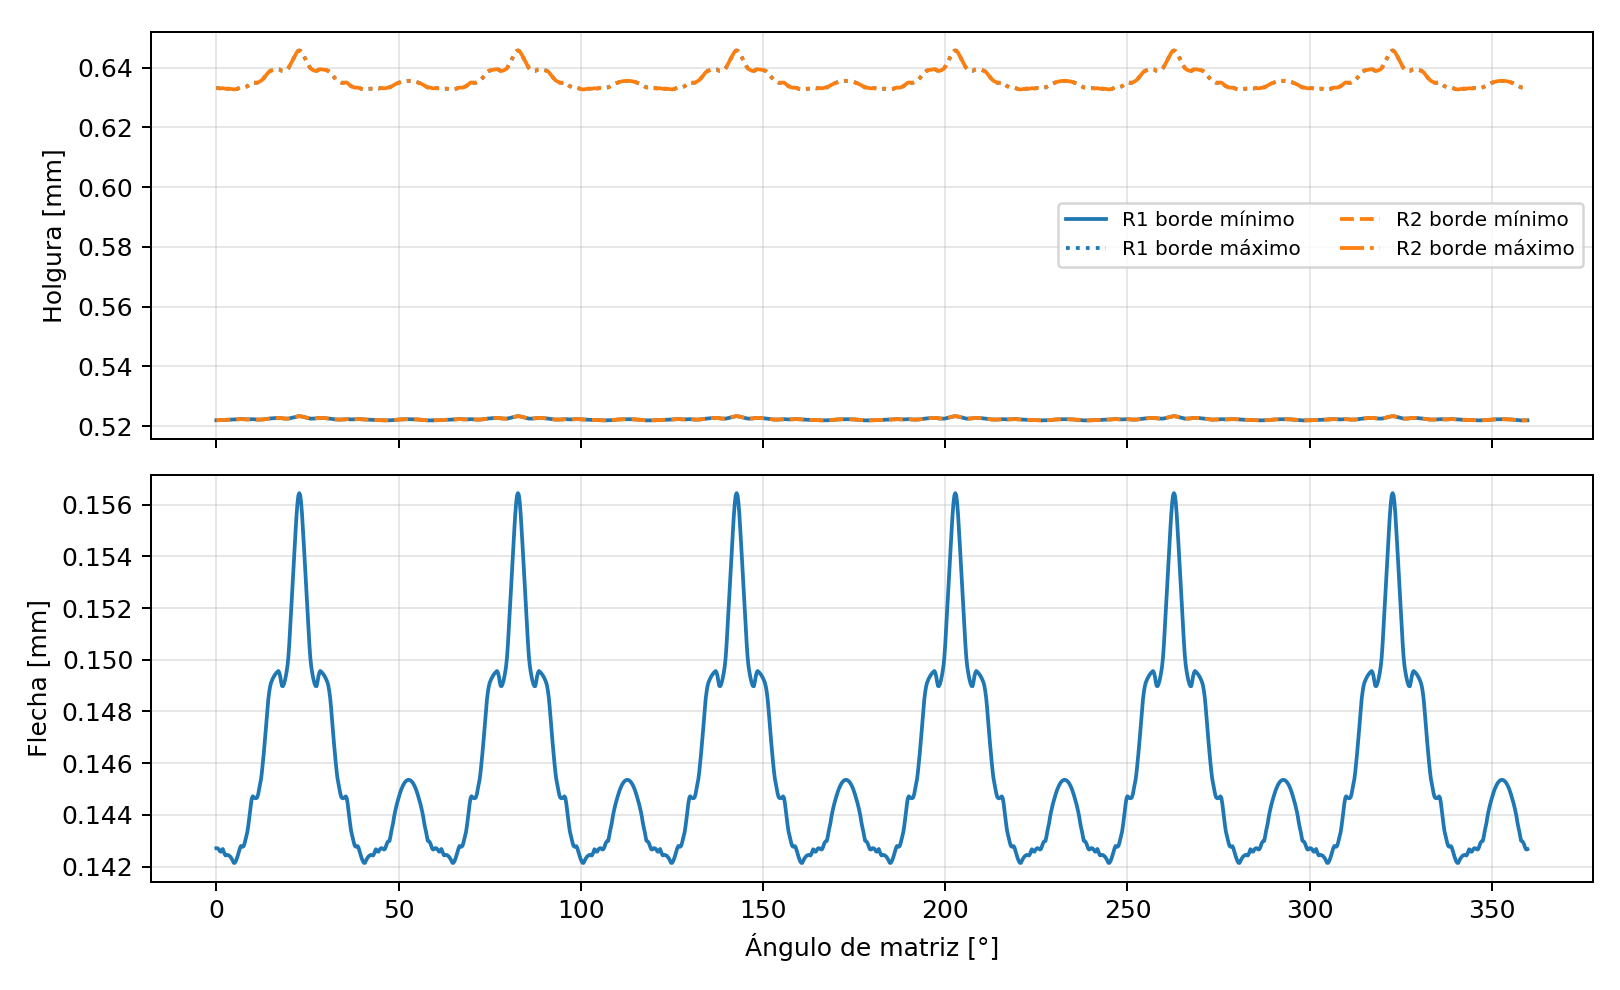
\includegraphics[width=.85\linewidth]{holguras_flecha.png}\end{center}
